\documentclass{article}
\usepackage{graphicx} % Required for inserting images
\usepackage{float}
\usepackage{tikz}
\title{OPTIMIZATION TECHNIQUES}
\author{Kavya Bajaj}
\date{Sem 3}

\begin{document}

\maketitle

\section{Introduction}

Optimization is the act of obtaining the best possible result under given circumstances or with minimum effort. It is used to improve the design, construction, and maintenance of engineering systems. Engineers make several technological and managerial decisions at different stages of a project to minimize cost, time, and resources while maximizing efficiency and performance.\vspace{0.6cm}

The ultimate goal of all such decisions is to minimize the effort required or maximize the desired benefit. Since the effort required or the benefit desired in any practical situation can be expressed as a function of certain decision variables, optimization can be defined as the process of finding the conditions that give the maximum or minimum value of a function.

\begin{figure}[H]
    \centering
    
    \includegraphics[width=1\linewidth]{image.png}
    \caption{Enter Caption}
    \label{fig:placeholder}
\end{figure}

It is so obvious that a point $x^*$ corresponds to the minimum value of $f(x)$. The same point also corresponds to the maximum value of $-f(x)$.




\begin{itemize}
    \item There is no single method available for solving optimization problems effectively. Hence, a number of optimization methods have been developed for solving different types of optimization problems.
\end{itemize}

\section*{Application of Optimization Problems in Engineering}

\begin{enumerate}
    \item Design of aircraft and aerospace structures for minimum cost.
    \item Design of civil engineering structures such as foundations, bridges, towers, and dams for minimum cost.
    \item Design of software for maximum profit.
\end{enumerate}

\section*{Statement of Optimization Problem}

An optimization problem can be stated as follows:

Find
\[
\mathbf{x}=(x_1,x_2,x_3,\ldots,x_n)^T
\]
such that it minimizes
\[
f(\mathbf{x})
\]
subject to the constraints
\[
g_j(\mathbf{x}) \leq 0,\qquad j=1,2,3,\ldots,m,
\]
and
\[
h_j(\mathbf{x}) = 0,\qquad j=1,2,3,\ldots,p.
\]

where $\mathbf{x}$ is an $n$-dimensional vector called the \textbf{design vector}.

\[
f(\mathbf{x}) \rightarrow \text{Objective function}
\]

\[
g_j(\mathbf{x}) \rightarrow \text{Inequality constraints}
\]

\[
h_j(\mathbf{x}) \rightarrow \text{Equality constraints}
\]





The problem stated in Eqn. is called a \textbf{constrained optimization problem}.

Some optimization problems do not involve any constraints and can be stated as unconstrained optimization problems.

Such problems are called \textbf{unconstrained optimization problems}.

\section*{Classical Optimization Technique}

Classical optimization techniques use differential calculus to determine the points of maxima and minima of continuous and differentiable functions. These techniques have limited scope in practical applications since practical applications involve objective functions that are not continuous and are not differentiable.

\vspace{0.5cm}

A function $f(x)$ is said to be increasing in an interval $(a,b)$ if the derivative

$f'(x)>=0$
then 
the function $f(x)$ is increasing 
\vspace{0.2cm}

or 
if $f'(x)<=0$
then 
the function $f(x)$. is decreasing 

\begin{center}

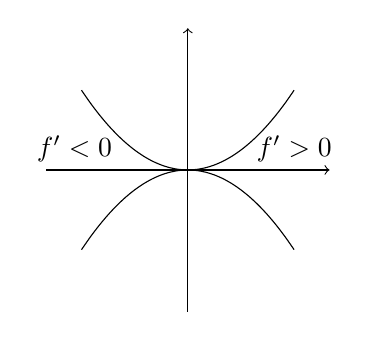
\begin{tikzpicture}[scale=0.9]
    % Axes
    \draw[->] (-2,0) -- (2,0);
    \draw[->] (0,-2) -- (0,2);

    % Increasing curve
    \draw[domain=-1.5:1.5,smooth,variable=\x]
        plot ({\x},{0.5*\x*\x});

    % Decreasing curve
    \draw[domain=-1.5:1.5,smooth,variable=\x]
        plot ({\x},{-0.5*\x*\x});

    \node at (-1.6,0.3) {$f'<0$};
    \node at (1.5,0.3) {$f'>0$};
\end{tikzpicture}
\end{center}


The point where the function changes its value from decreasing to increasing is a \textbf{local minimum}.

\begin{itemize}
    \item The point where the function changes its value from increasing to decreasing is a \textbf{local maximum}.
    
    \[
    f''(x) < 0
    \]
\end{itemize}

\section*{Local Extrema (Optimum)}

Local extrema points are the points where

\[
f'(x)=0,
\]

or where $f'(x)$ is undefined, or at one of the end points of the domain.

\vspace{0.5cm}

\subsection*{Critical Point}

A point at which

\[
f'(x)=0
\]

is called a \textbf{critical point}.

A point at which

\[
f''(x)=0
\]

is called an \textbf{inflection point}.





\title{Optimization Techniques \\ 10\textsuperscript{th} July}
\date{}
\maketitle

\section*{Find the points of minimum and maximum of the following function}

\[
f(x)=2x^3-9x^2+12x+6
\]

\subsection*{Solution}

Differentiate the function:

\[
f'(x)=6x^2-18x+12
\]

Factorizing,

\[
f'(x)=6(x^2-3x+2)
\]

\[
=6(x-1)(x-2)
\]

Therefore,

\[
f'(x)=0
\]

for

\[
x=1,\;2
\]

Hence, the critical points (C.P.) are

\[
(1,\;2)
\]

---

### Sign of $f'(x)$

\[
\begin{array}{c|ccc}
x & (-\infty,1) & (1,2) & (2,\infty)\\
\hline
f'(x) & + & - & +
\end{array}
\]

Therefore,

- Increasing on $(-\infty,1)$
- Decreasing on $(1,2)$
- Increasing on $(2,\infty)$

Hence,

- At $x=1$, the function changes from increasing to decreasing.

\[
\boxed{\text{Local Maximum}}
\]

- At $x=2$, the function changes from decreasing to increasing.

\[
\boxed{\text{Local Minimum}}
\]

---

### Maximum Point

Substitute $x=1$ into $f(x)$.

\[
f(1)=2(1)^3-9(1)^2+12(1)+6
\]

\[
=2-9+12+6
\]

\[
=11
\]

Therefore,

\[
\boxed{\text{Local Maximum at }(1,11)}
\]

---

### Minimum Point

Substitute $x=2$ into $f(x)$.

\[
f(2)=2(2)^3-9(2)^2+12(2)+6
\]

\[
=2(8)-9(4)+24+6
\]

\[
=16-36+24+6
\]

\[
=10
\]

Therefore,

\[
\boxed{\text{Local Minimum at }(2,10)}
\]

\vspace{1cm}

\textbf{Note:}

If the domain is changed from

\[
(-\infty,\infty)
\]

to

\[
[-1,4],
\]

then we must also evaluate the function at the endpoints:

\[
f(-1)\quad\text{and}\quad f(4)
\]

and compare these values with

\[
f(1)=11,\qquad f(2)=10
\]

to determine the absolute maximum and absolute minimum on the interval.


\section*{Absolute Extrema on the Interval \texorpdfstring{$[-1,4]$}{[-1,4]}}

Evaluate the function at the critical points and the endpoints:

\[
f(-1), \qquad f(1)=11, \qquad f(2)=10, \qquad f(4)
\]

Hence,

\[
\boxed{\text{Absolute Minimum at }x=-1 \text{ and }x=2}
\]

\[
\boxed{\text{Absolute Maximum at }x=1 \text{ and }x=4}
\]

\vspace{0.5cm}

\section*{Necessary and Sufficient Conditions for Local Extreme Values}

\subsection*{1. Necessary Condition}

If a function $f(x)$ is defined on an interval

\[
a \le x \le b
\]

and has a local minimum or maximum at

\[
x=x^*,
\]

where

\[
a<x^*<b,
\]

and if the first derivative exists at $x=x^*$, then

\[
\boxed{f'(x^*)=0.}
\]

\vspace{0.5cm}

\subsection*{2. Subsient Condition}

Suppose

\[
f'(x^*)=0,\qquad
f''(x^*)=0,\qquad
f'''(x^*)=0,\quad \ldots,\quad
f^{(n-1)}(x^*)=0,
\]

but

\[
f^{(n)}(x^*)\neq0.
\]

Then,

\begin{enumerate}
    \item $f(x)$ has a \textbf{minimum} value at $x=x^*$ if
    \[
    f^{(n)}(x^*)>0
    \]
    and $n$ is even.

    \item $f(x)$ has a \textbf{maximum} value at $x=x^*$ if
    \[
    f^{(n)}(x^*)<0
    \]
    and $n$ is even.

    \item $f(x)$ has \textbf{neither a maximum nor a minimum} if $n$ is odd.
\end{enumerate}

\section*{2. Determine the Maximum and Minimum Values of the Function}

Given,

\[
f(x)=2x^3-9x^2+12x+6
\]

The second derivative is

\[
f''(x)=12x-18.
\]

To find the point of inflection,

\[
12x-18=0
\]

\[
6(2x-3)=0
\]

\[
x=\frac{3}{2}.
\]

\vspace{0.5cm}

\textbf{Second Derivative Test}

We evaluate the second derivative at the critical points obtained previously.

At $x=1$,

\[
f''(1)=12(1)-18=-6<0.
\]

Hence,

\[
\boxed{x=1 \text{ is a local maximum}.}
\]

Also,

\[
f(1)=11.
\]

Therefore,

\[
\boxed{\text{Local maximum value}=11.}
\]

\vspace{0.5cm}

At $x=2$,

\[
f''(2)=12(2)-18=6>0.
\]

Hence,

\[
\boxed{x=2 \text{ is a local minimum}.}
\]

Also,

\[
f(2)=10.
\]

Therefore,

\[
\boxed{\text{Local minimum value}=10.}
\]

\hrulefill

\section*{4. Find the Local Maximum and Minimum Values}

Given,

\[
f(x)=x^6-6x^5+9x^4
\]

Differentiate the function:

\[
f'(x)=6x^5-30x^4+36x^3.
\]

Let

\[
f'(x)=0.
\]

Then,

\[
6x^5-30x^4+36x^3=0,
\]

or

\[
x^5-5x^4+6x^3=0.
\]

Factorizing,

\[
x^3(x^2-5x+6)=0,
\]

\[
x^3(x-2)(x-3)=0.
\]

Hence, the critical points are

\[
\boxed{x=0,\;2,\;3.}
\]

\vspace{0.5cm}

The second derivative is

\[
f''(x)=30x^4-120x^3+108x^2.
\]

Factorizing,

\[
f''(x)=6x^2(5x^2-20x+18).
\]

Now evaluate the second derivative at the critical points.

For \(x=0\),

\[
f''(0)=0.
\]

Since the second derivative is zero, the second derivative test is inconclusive.

\vspace{0.5cm}

For \(x=2\),

\[
f''(2)=6(2)^2\left[5(2)^2-20(2)+18\right]
\]

\[
=24(20-40+18)
\]

\[
=24(-2)
\]

\[
=-48<0.
\]

Hence,

\[
\boxed{x=2 \text{ is a local maximum}.}
\]

\vspace{0.5cm}

For \(x=3\),

\[
f''(3)=6(3)^2\left[5(3)^2-20(3)+18\right]
\]

\[
=54(45-60+18)
\]

\[
=54(3)
\]

\[
=162>0.
\]

Hence,

\[
\boxed{x=3 \text{ is a local minimum}.}
\]

\vspace{0.5cm}

The third derivative is

\[
f'''(x)=120x^3-360x^2+216x.
\]

Evaluating at \(x=0\),

\[
f'''(0)=0.
\]

\section*{5. Find the Local Maximum and Minimum Values}

Given,

\[
f(x)=12x^5-45x^4+40x^3+5.
\]

Differentiate the function:

\[
f'(x)=60x^4-180x^3+120x^2.
\]

Let

\[
f'(x)=0.
\]

Then,

\[
60x^4-180x^3+120x^2=0,
\]

or

\[
x^2(x^2-3x+2)=0.
\]

Factorizing,

\[
x^2(x-2)(x-1)=0.
\]

Hence, the critical points are

\[
\boxed{x=0,\;1,\;2.}
\]

The second derivative is

\[
f''(x)=240x^3-540x^2+240x.
\]

Evaluating the second derivative at the critical points:

For \(x=0\),

\[
f''(0)=0.
\]

Hence, the second derivative test is inconclusive.

For \(x=1\),

\[
f''(1)=240-540+240
=-60<0.
\]

Hence,

\[
\boxed{x=1 \text{ is a local maximum}.}
\]

Also,

\[
f(1)=12.
\]

For \(x=2\),

\[
f''(2)=240(8)-540(4)+240(2)
=1920-2160+480
=240>0.
\]

Hence,

\[
\boxed{x=2 \text{ is a local minimum}.}
\]

Also,

\[
f(2)=-11.
\]

The third derivative is

\[
f'''(x)=720x^2-1080x+240.
\]

Evaluating at \(x=0\),

\[
f'''(0)=240.
\]

\hrulefill

\section*{Practice Problems}

Find the local maximum and minimum values of the following functions:

\begin{enumerate}
    \item
    \[
    f(x)=4x^3-8x^2+27x-7.
    \]

    \item
    \[
    f(x)=x^3-3x+6.
    \]

    \item
    \[
    f(x)=3x^4-4x^3-24x^2+48x+115.
    \]

    \item
    \[
    f(x)=\sin x,\qquad
    -\frac{\pi}{2}\le x\le\frac{5\pi}{6}.
    \]
\end{enumerate}

\hrulefill

\section*{Question}

For what values of \(a\) and \(b\) will the function

\[
f(x)=ax^3-bx^2+36x
\]

have a minimum at \(x=3\) and a maximum at \(x=1\,\) ?

\vspace{0.5cm}
\hrulefill
\vspace{0.5cm}



\section*{Single Variable Optimization Methods}

\begin{itemize}
    \item Analytical Method
    \item Direct Search Method
    \item Gradient Based Method
\end{itemize}

\subsection*{Direct Search Method}

\begin{itemize}
    \item \textbf{Bracketing Method}
    \begin{enumerate}
        \item Exhaustive Search Method
        \item Bounding Phase Method
    \end{enumerate}

    \item \textbf{Region Elimination Method}
    \begin{enumerate}
        \item Interval Halving Method
        \item Fibonacci Search Method
        \item Golden Search Method
    \end{enumerate}

    \item \textbf{Point Estimation Method}
    \begin{enumerate}
        \item Successive Quadratic Elimination Method\\
        (Powell's Method)
    \end{enumerate}
\end{itemize}

\hrulefill

\section*{Exhaustive Search Method}

It searches the optimum in a given interval

\[
(a,b).
\]

\subsection*{Algorithm}

\textbf{Step 1:}

Set

\[
x_1=a,
\]

\[
\Delta x=\frac{b-a}{n},
\]

where \(n\) is the number of intervals into which the given interval is divided.

Next,

\[
x_2=x_1+\Delta x,
\]

\[
x_3=x_2+\Delta x.
\]

\textbf{Step 2:}

Evaluate

\[
f(x_1),\;f(x_2),\;\text{and}\;f(x_3).
\]

If

\[
f(x_1)\geq f(x_2)\leq f(x_3),
\]

then the minimum point lies in the interval

\[
(x_1,x_3).
\]

Otherwise, terminate.


\textbf{Else:}

Set

\[
x_1=x_2,\qquad
x_2=x_3,\qquad
x_3=x_2+\Delta x
\]

and go to \textbf{Step 3}.

\bigskip

\textbf{Step 3:}

Check whether

\[
x_3<b.
\]

\begin{itemize}
    \item If \textbf{Yes}, go to \textbf{Step 2}.
    \item If \textbf{No}, no minimum exists in the interval
    \[
    (a,b),
    \]
    or a boundary point is the minimum.
\end{itemize}

\hrulefill

\textbf{Note:}

\begin{enumerate}
    \item The length of the final interval obtained by this method is

    \[
    2\Delta x
    =\frac{2(b-a)}{n}.
    \]

    \item To obtain a 3-decimal accuracy, choose the interval length as

    \[
    0.001.
    \]

    For 4-decimal accuracy, choose

    \[
    0.0001,
    \]

    and so on.
\end{enumerate}

\hrulefill

\section*{Example}

Find the minimum of

\[
f(x)=x^2+\frac{54}{x},
\]

in the interval

\[
(2,5)
\]

using the Exhaustive Search Method. Choose

\[
n=10.
\]

Also find the analytical solution. What should be the value of \(n\) if 3-decimal accuracy is required?

\subsection*{Analytical Solution}

Given,

\[
f(x)=x^2+\frac{54}{x}.
\]

First derivative:

\[
f'(x)=2x-\frac{54}{x^2}.
\]

For stationary points,

\[
f'(x)=0.
\]

Therefore,

\[
2x=\frac{54}{x^2}
\]

\[
2x^3-54=0
\]

\[
x^3=27
\]

\[
\boxed{x=3.}
\]

Now,

\[
f''(x)=2+\frac{108}{x^3}.
\]

At \(x=3\),

\[
f''(3)=2+\frac{108}{27}
\]

\[
=2+4
\]

\[
=6>0.
\]

Hence,

\[
\boxed{x=3 \text{ is a point of local minimum}.}
\]

Minimum value:

\[
f(3)=3^2+\frac{54}{3}
\]

\[
=9+18
\]

\[
=27.
\]

Therefore,

\[
\boxed{\text{Minimum value}=27 \text{ at } x=3.}
\]

\end{document}

